This section is divided into two parts. In \autoref{sec:method-T-reX_tool}, we describe the T-reX tool, in \autoref{sec:method-case_study}, we describe the methodology used to calculate the waste and material inventory footprints in a case study of 6 Li-ion batteries.

\subsection{The T-reX tool}\label{sec:method-T-reX_tool}

\subsubsection{Computational framework}
\label{sec:method-T-reX_tool}

Developed in the Python programming language, T-reX extends the brightway LCA framework, utilising the components \texttt{bw2data}, \texttt{bw2calc}, and \texttt{bw2io}~\citep{mutel2017brightway}. Additionally, the \texttt{wurst} package---which can expand entire databases into a list of exchanges---is used to facilitate database searching and data transformation at the exchange level~\citep{mutel2017wurst}. Integration with the \texttt{premise} package~\citep{sacchi2022premise}---which integrates the projections of integrated assessment models (IAMs) into current LCA databases---enables the user to easily create and manipulate prospective LCA databases. T-reX is also compatible with \texttt{ActivityBrowser}~\citep{steubing2020activitybrowser}---an open-source graphical user interface for LCA---after running T-reX, the manipulated databases and the 'pseudo' LCIA methods created by T-reX can be used in the accustomed way. The T-reX tool is installable via the Python Package Index (PyPI)~\citep{mcdowall2023T-reXpipy} and is open source under the CC-0 licence. The full source code for the T-reX tool is indexed on Zenodo~\citep{mcdowall2023T-reXzenodo} and under further development in the GitHub repository~\citep{mcdowall2024T-reXgithub}. T-reX is designed to be used with ecoinvent databases~\citep{ecoinvent2016version3}, but could be adapted to other databases by changing the search criteria. Currently, it has been tested with all available system models of ecoinvent 3.5--3.10~\citep{ecoinvent2016version3}.

T-reX can be used directly from the command line, or imported as a Python module, in which case, the user can access the individual functions and modules. In the simplest case, the user can run the program with the default settings, which will calculate the waste and material footprint of the ecoinvent database. The user can also customise T-reX to calculate the waste and material inventory footprints of a custom database, or a prospective database based on future scenarios by implementing \texttt{premise} with an included module.

The supplementary information [ADD LINK] contains the full metadata of T-reX tool, along with a list of the constituent modules of the T-reX tool, a description of their functions and a detailed computational workflow. Further details can be found in the user guide and documentation~\citep{mcdowall2023T-reXdocs}.

\subsubsection{Functionality and purpose}

T-reX is a Python package that allows one to produce LCA databases---both current and prospective---that are manipulated to facilitate the calculation of waste and material inventory footprints in the supply chain of any activity in the same was as standard LCIA methods. 

If desired, prospective databases can be custom-defined by the user or constructed with the projections of the integrated assessment models such as IMAGE~\citep{stehfest2014image} and REMIND~\citep{remind2020model}, which offer a range of options aligned with the Shared Socioeconomic Pathways (SSPs)~\citep{ssp2020ghg} that can be paired with a variety of mitigation scenarios.

Subsequent expansion of the databases into lists of exchanges allows relevent material and waste flows to be identified and categorised. The search queries are tailored to the specific database and the user can easily modify them to suit their needs. The categories defined in the configuration are used to create T-reX's `pseudo LCIA' methods that are indicators of aggregated technosphere demand. The exchange editing function of T-reX then takes each list of exchanges and appends to the relevent activity a copy of the technosphere exchange as `pseudo-biosphere' exchange that matches the `pseudo LCIA' method.

In the default configuration, there are 10 waste categories which are further divided by their unit of measurement (kilograms and cubic meters) to create a total of 20 waste methods. The waste categories include incineration, recycling, and total waste, and are listed in the supplementary information [ADD LINK]. One advantage of T-reX is that is is able to identify of waste exchanges that would otherwise be `consumed' by a treatment process and not leave the technosphere. Since `waste is not a service'~\citep{guinee2021wasteisnotaservice}, a characterisation factor of -1 is applied to the waste footprint methods (with the exception of CCS exchanges), changing the perspective from `waste consumed by treatment' to `waste generated by the activity'.

In addition to the waste categories, the \texttt{queries\_materials} module defines the material demand categories, which are based on the EU Critical Raw Materials (CRM) list for 2023~\citep{eu2023crmstudy}. The CRM list is a list of 30 materials that are considered critical to the EU economy and are at risk of supply disruption. Further materials of interest to the authors were added to the search list, including helium, electricity, petroleum, sand, water, and natural gas. The identity of the materials considered and their categorical groupings are easily customisable by the user. The full list of 59 materials included in the default configuration is provided in the supplementary material [ADD LINK].

The logic for the identification of material exchanges with the T-reX tool differs from that used to identify waste exchanges in that the search queries are based on the names of the so-called relevant `market activities' for the material of interest. A useful feature of the T-reX tool is that, in cases where there are several markets for one material or material group, the program can easily aggregate these exchanges. For example, exchanges with markets for the rare-earth-elements (REEs) `market for cerium', `market for dysprosium', `market for erbium', etc.\ can be aggregated into a single indicator category for REEs. Similarly, the total demand for all critical raw materials (CRMs) can be easily calculated in the same manner. 

As discussed in the introduction~\ref{sec:introduction} there are some existing material demand methods in the standard LCIA method sets, including the `crustal scarcity indicator' (which provides only an aggregated, abstracted endpoint)~\citep{arvidsson2020csi} and the (deprecated) EDIP 2003 material use indicators (which provide endpoints in fundamental units)~\citep{hauschild2003edip}. In these methods, the material demand is calculated based on the total mass that is extracted from the environment, thus, their focus is essentially solely on the mining-related exchanges that bring these materials from the biosphere into the technosphere. In the T-reX tool, however, the accounting for material demand is based on exchanges solely within the technosphere. This offers a different perspective, allowing for the estimation of overall supply-chain material demands that consider the entire life cycle of an activity, including non-direct impacts on the market such as co-production of other materials. Consider a demand for an activity containing a metal, for example; while the existing material use methods allow one to calculate the total mass of that metal that is extracted from the environment, the T-reX tool can provide insight into the broader supply-chain impacts of the demand for this metal. If the production other materials are attributed to the production of this metal, these would appear as negative material demands in the T-reX results---supply chain pressure for one material can result in lessening of supply chain pressure for another. In the results of the Li-ion battery case study in \autoref{sec:results-case_study}, we will see that this is indeed the case for the demand for nickel, which, because of such effects, is counter-intuitively negative despite the presence of nickel in the final products.

% \subsubsection{Theoretical basis}

% XXX

\subsubsection{T-reX tool workflow}

The workflow of the T-reX tool is divided into several modules, each of which performs a specific function. The modules are designed to be used in a specific order, but the user can also use them individually to perform specific tasks. The standard workflow is as follows:

\begin{enumerate}
    \item Configuration of waste and material exchange categorisation (optional)
    \item Generation of prospective LCA databases (optional)
    \item Database expansion---to create a list of all exchanges in the database
    \item Identification and categorisation of exchanges
    \item Creation of `pseudo-biosphere' databases
    \item Creation of `pseudo-LCIA' methods to calculate waste and material inventory footprints
    \item Exchange editing---whereby the technosphere exchange is mirrored as a `pseudo-biosphere' exchange
    \item Database verification
\end{enumerate}

This workflow creates one or more manipulated LCA databases that can then be used to calculate the waste and material inventory footprints of activities in the same way as standard LCIA calculations.

A generic flowchart of the T-reX tool workflow is presented in \autoref{fig:methods-flowchart}. The supplementary material [ADD LINK] contains a more detailed computational flowchart.

\begin{figure}[H]
    \centering
    \caption{Workflow of the T-reX tool. Application of T-reX to one or more LCA databases creates a brightway project with customised methods and activities that can be used to calculate the waste and material inventory footprints.}
    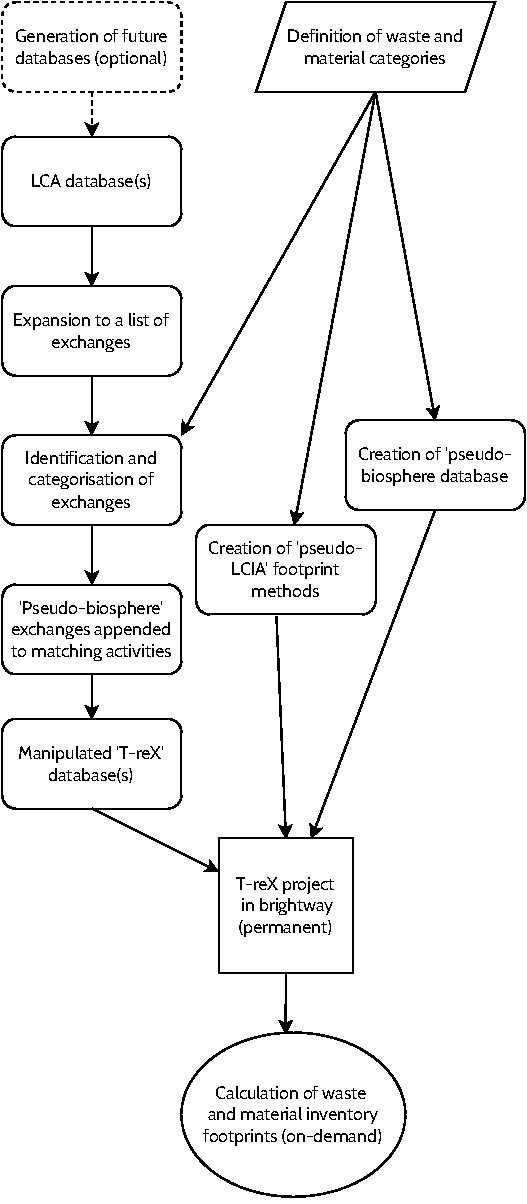
\includegraphics[width=0.5\linewidth]{figures/T-reX_method.pdf}
    \label{fig:methods-flowchart}
\end{figure}


\subsection{Case Study Methodology}\label{sec:method-case_study}

We investigated five types of Li-ion batteries, each represented by specific market activities:
\begin{itemize}[itemsep=0pt]
    \item Li-ion, NMC111, rechargeable, prismatic
    \item Li-ion, LiMn2O4, rechargeable, prismatic
    \item Li-ion, NCA, rechargeable, prismatic
    \item Li-ion, NMC811, rechargeable, prismatic
    \item Li-ion, LFP, rechargeable, prismatic
\end{itemize}

In addition to the waste and material inventory footprint methods created by the T-reX tool, the following standard LCIA methods were applied for comparison:

\begin{itemize}[itemsep=0pt]
    \item ReCiPe 2016 v1.03, midpoint (I)
    \item EF v3.0 no LT
    \item EDIP 2003 no LT
    \item Crustal Scarcity
\end{itemize}

The primary source of life cycle inventory data for this case study was ecoinvent 3.9.1 cutoff. Additionally, the T-reX tool was used to create prospective database sets using the \mbox{REMIND} model with the following Representative Concentration Pathways (RCPs):
\begin{itemize}
    \item SSP2-base: representing an approximate 3.5°C increase in global temperatures to 2100
    \item SSP2-PkBudg500: representing the achievement of Paris climate goals, ca. 1.3°C increase to 2100
\end{itemize}

For each pathway, databases were created with texttt{premise}~\citep{sacchi2022premise} and processed with the T-reX tool over the time series: 2020, 2040, 2060, 2080, 2100.

\subsubsection{Calculations}
For each combination of activity, method, and database, a single score `LCIA' was calculated along with details of the top contributing processes. Additionally, for the Waste and Material Footprint methods, a contribution analysis was performed. This involved utilizing the \texttt{bwa.compare\_activities\_by\_grouped\_leaves} function from the \texttt{brightway2\_analyzer} package~\citep{mutel2016brightway2analyzer}, an additional component of the Brightway2 LCA framework. This function performs graph traversal on the impact matrix of the LCA object to a specified cutoff and groups the resulting leaves by their CPC codes. This provides insight into the products and sectors in the supply chain of the activity that carry the most responsibility for the final footprint.


